\documentclass[modern]{aastex62} 
\setlength{\parskip}{\baselineskip}

%\usepackage{graphicx}
\usepackage{amsmath}
\usepackage{mathtools}
\usepackage[normalem]{ulem}

\newcommand{\transpose}[1]{{#1}^{\!\mathsf T}}
\newcommand{\given}{\,|\,}
\renewcommand{\det}[1]{||{#1}||}
\newcommand{\abs}[1]{|{#1}|}
\DeclareMathOperator{\trace}{Tr}

\newcommand{\counts}{C}
\newcommand{\countrate}{\hat{C}}
\newcommand{\exptime}{t_{\mathrm{exp}}}
\newcommand{\model}{\mathcal{M}}
\newcommand{\psf}{\mathcal{P}}
\newcommand{\prf}{\mathcal{R}}
\newcommand{\qe}{Q}
\newcommand{\scene}{\mathcal{S}}
\newcommand{\like}{\mathcal{L}}
\newcommand{\normal}{\mathcal{N}}
\newcommand{\dx}{\Delta_x}
\newcommand{\dy}{\Delta_y}


%\makeatletter
%\renewcommand*\env@matrix[1][c]{\hskip -\arraycolsep
%  \let\@ifnextchar\new@ifnextchar
%  \array{*\c@MaxMatrixCols #1}}
%\makeatother


\begin{document}
%\title{Image Forward Modeling Techniques}
\author{Image Forward Modeling Techniques}

%\begin{center}
%\today
%\end{center}

\section{Notation}
I try to use script letters for probability distributions (e.g. $\scene$), with parameters as greek letters (e.g. $\gamma$).
Draws from a distribution are denoted by $\sim$.
Functions are given uppercase italic letters (e.g. $\qe$).
Scalar variables are lowercase italic letters.
Vector variables are \sout{bolded} lowercase.
Matrices are \sout{bolded} uppercase.

\section{Introduction}
We want a generative model for the image(s) that can be plugged into a
likelihood function and an MC sampling scheme. Therefore the goal is to go from
the scene to counts in pixels. The basic function that we are trying to compute
(efficiently) is:
\begin{eqnarray}
\countrate_n & = & F_n(\gamma, \beta)
\end{eqnarray}
where 
$\countrate_n$ is the expected counts in the $n$th pixel,
there are $n=1,2,...N$ pixels,
$\gamma$ are the parameters describing the instrument (PSF, PRF, distortions, etc.),
and ${\bf \beta}$ are the parameters describing the scene (i.e. source positions and shapes).
In the end we will want to calculate
\begin{eqnarray}
\like(\{\counts_n\} \given \{\exptime \, \countrate_n\}) & = & \prod_n \, \frac{e^{-\exptime \, \countrate_n} \, (\exptime \, \countrate_n)^{\counts_n}} {\counts_n !}
\end{eqnarray}
(or probably the Gaussian likelihood since there will be plenty of counts.)
Ideally we will also be able to efficiently calculate (analytically) the
gradients of the ln-likelihood with respect to any of the source (and perhaps
even instrument) parameters. Analytic gradients can vastly accelerate both
optimization and MCMC bayesian inference.

Here's the Gaussian likelihood and its derivatives
\begin{eqnarray}
R_n & = & C_n - I_n(\theta) \nonumber \\
\chi_n & = & R_n / \sigma_n \nonumber \\
\ln \like(C \given \theta) & = & -\frac{1}{2} \sum_n \chi_n^2 \nonumber \\
\frac{\partial \ln \like}{\partial \theta_k} & = & \sum_n \frac{R_n}{\sigma_n^2} \frac{\partial I_n}{\partial \theta_k} 
\end{eqnarray}
where $\theta = \{\beta, \gamma\}$

\section{Full Problem}

What's really happening from a photon's point of view (sort of)? First it comes
from a distribution $\scene(\alpha, \delta [, \nu] \given \beta)$ which we take
to be the intensity distribution on the sky, or the \emph{scene}, parameterized
by $\beta$. It then travels through the the atmosphere (if there is one), then
the telescope optics, finally reaching the detector plane. During this travel
the photon is diffracted and refracted, so that its position is now in iteself a
PDF (called the point spread function, $\psf$). Upon striking the detector the
wavefunction is collapsed and the detector position is drawn from this PDF, with
some probability related to the quantum efficiency of the detector at that
position (and the reflectivity of the optics, etc.). One must also consider gaps
in the detector, and intrapixel sensitivity variations, which might be folded
into a spatially dependent QE or pixel response function, or alternatively
combined with the PSF somehow. The mapping from the celestial position to the
detector plane depends on the distortion of the optics and the aforemention
probabilistic draw from $\psf$. This can all be represented by 
\begin{eqnarray}
\label{eqn:photon}
\alpha_j, \delta_j [, \nu_j] & \sim & \scene(\beta)\\
x_j, y_j & = & D(\alpha_j, \delta_j)  \nonumber \\ 
\Delta x_j, \Delta y_j & \sim & \psf(\gamma, x_j, y_j [, \nu_j]) \nonumber \\
\countrate_n & \propto & \lim_{J\to\infty} \frac{1}{J} \sum^J_{j=1} \qe_n(x_j+ \Delta x_j, y_j + \Delta y_j [, \nu_j]) \nonumber
\end{eqnarray}
where $\scene$ is the sky instensity distribution in celestial coordinates 
and depends on parameters $\beta$,
$\alpha_j$ and $\delta_j$ are the coordinates of the $j$th draw from $\scene$,
$D$ is the mapping from celestial to detector coordinates $(x, y)$ including distortion,
$\psf$ is the point-spread-function in detector coordinates and depends on parameters $\gamma$ as well as the detector location,
$\Delta x_j, \Delta y_j$ are draws from $\psf$,
$\qe_n(x, y)$ is the detector quantum efficiency of the $n$th pixel at location $(x, y)$ (usually something close to a bivariate boxcar),
and $\countrate_n$ is the expected countrate in pixel $n$ per unit time and total number of photons due to celestial sources (i.e. excluding detector background.)
The scene can be expressed as a sum of individual source distributions $\scene =
\sum_{m=1}^M \scene_m$. In what follows we will drop $\nu$ from consideration,
assuming that $\qe(\nu)$ is a constant that can be factored out.


In the limit of infinite exposure time (or very many photons), we can replace
the sum of a large number of draws with integrals to obtain the expected count
rate.
\begin{eqnarray}
\label{eqn:psf_convolve}
\model(x, y \given \gamma, \beta) & = & \iint \, dx' \, dy' \, \psf(x - x', y-y' \given \gamma, x', y') \, \scene( D^{-1}(x', y') \given \beta) \\
\countrate_n & = & \iint_{A_n} \, dx \, dy \, \qe_n(x, y) \, \model(x, y \given \gamma, \beta) \nonumber
\end{eqnarray}
where $A_n$ is the region of the $n$th pixel, 
$\model$ is the PSF-convolved scene,
$\psf$ is the point-spread function (which depends on the input position of the photon),
and $D$ is the mapping from sky coordinates to detector coordinates, including distortions.

One question is whether it makes more sense to think of the pixels as rectangles
in detector coordinates and project the scene into these coordinates as we have
done above, or to project the pixel boundaries (and $\psf$ and $\qe$) into
celestial coordinates. This probably depends on the form of $D$ and on how the
$\qe$ and $\psf$ functions are determined. Nevertheless, by switching the order
of integration we can write
\begin{eqnarray}
\label{eqn:prf_integral}
\prf_n(x', y' \given \gamma) & = & \iint_{A_n} \, dx \, dy \, \qe_n(x, y) \, \psf(x' - x, y' - y \given \gamma, x, y) \\
\countrate_n & = & \iint \, dx' \, dy' \, \prf_n(x', y' \given \gamma) \, \scene( D^{-1}(x', y') \given \beta) \nonumber
\end{eqnarray}
where $\prf_n(x', y')$ gives the response of a pixel to a point source at detector coordinates $(x', y')$ including the effect of the pixel-averaged PSF.
This form can be easier to compute, since this pixel response function (PRF) can
be specified beforehand, or at least once approximated includes the annoying
integral over $A_n$.

These convolutions and integrals can be analytically intractable, or time
consuming. This is especially true the case of complicated forms for $\psf$,
$\prf$, $\scene$ or the function $D$. Much of the guts of any forward modeling
algorithm will be concerned with approximating this integral, especially in a
way that yields analytic gradients.


\section{Approximation by Gaussian Mixtures (and Subgridding)}

One method to make the integrals more tractable is to calculate $\prf$ and
$\scene$ on fine grids and calculate \ref{eqn:prf_integral} directly on this
grid. The grid has to be fine enough that the integral can be approximated by a
sum; that is, the grid must fully sample the PRF and the scene.
\begin{eqnarray}
\label{eqn:prf_grid}
\countrate_{n'} & \approx & \sum_{i,j} \prf_{n'}(x_i, y_j \given \gamma) \, \scene( D^{-1}(x_i, y_j) \given \beta) \nonumber
\end{eqnarray}
It can then be rebinned to produce the actual pixel $\countrate_n$.
One approach to obtain gradients with respect to the parameters $\gamma, \beta$ is to further approximate $\prf$ and $\scene$ by mixtures of Gaussians.
This allows one to write the countrate as 
\begin{eqnarray}
\prf_{n'}(x, y \given \gamma)  & = & \sum_k w_k(\gamma) \, \normal(x, y \given \mu_{k, n'}(\gamma), \Sigma_k(\gamma)) \\
\scene(x, y \given \beta) & = & \sum_\ell w_\ell(\beta) \, \normal(D^{-1}(x, y) \given \mu_\ell(\beta), \Sigma_\ell(\beta)) \nonumber \\
\countrate_{n'} & = & \sum_{i,j}\sum_{k} \, w_k \, \normal(x_i, y_j \given \mu_{k, n'}, \Sigma_{k, n'}) \, \sum_\ell w_\ell \, \normal(D^{-1}(x_i, y_j) \given \mu_{\ell}, \Sigma_{\ell}) \nonumber
\end{eqnarray}
where $\normal(a, b \given \mu, \Sigma)$ is the bivariate normal distribution with location $\mu$ and covariance matrix $\Sigma$ evaluated at $(a, b)$.


The drawbacks here are:
   1) evaluating large numbers of exponentials
   2) finding nice representations of parameterized scenes and PRFs in terms of mixtures of Gaussians such that the gradients of the Gaussian parameters with respect to the scene parameters $\beta$ are relatively simple
   3) limited accuracy of the mixture of Gaussians approximation.
   4) Gaussians do not have a defined maximum frequency and are thus always undersampled to some degree by any grid.
   5) Location dependent PSF or PRF can be unwieldy.
One could also replace the $\prf$ mixture of Gaussians with the polynomial or spline approximation discussed below.
I think the Tractor does something like \ref{eqn:psf_convolve} but with a $\delta$-function $\qe$, in which case the PSF and the PRF are equivalent.

\subsection{Undersampling}
One difficulty in this method is accounting for undersampling of the PRF by the pixels.
The JWST F090W has pixels $\sim$ FWHM of the PSF.
One strategy is to make calculations on subpixel grids and then sum/rebin.
However, this entails quite a bit of extra computation (and gradients have to be tracked).
Another option is to account for the undersampling by using a second order approximation to the integral of the gaussian over a square pixel.
In Figure \ref{fig:undersample} there is a demonstration of the accuracy of this apprximation compared to a highly oversampled and rebinned calculation, for a particular subpixel shift and a gaussian PSF with FWHM of 1 pixel.
If this proves insufficiently accurate, it would not be that difficult (except in compute time) to implement a mild oversampling scheme to improve the accuracy.

Here is the math for the 2nd-order approximation to a gaussian centered at $(x_s, y_s)$ with amplitude $A_s$ and covariance matrix $\Sigma_s$
\begin{eqnarray}
I(x_p, y_p)   & = & A_s \, h \, e^{g } \\
\dx, \dy & = & x_p - x_s, y_p - y_s  \nonumber\\
g     & = & -\frac{1}{2} \, (\dx \, V_{x} + \dy \, V_y) \nonumber \\
h     & = & 1 + \frac{1}{24} \, (V_x^2 + V_y^2 - F_{xx} - F_{yy}) \nonumber \\
V_x  & = & F_{xx} \, \dx + F_{xy} \, \dy  \nonumber \\
V_y  & = & F_{yy} \, \dy + F_{xy} \, \dx \nonumber \\
F & = & \Sigma^{-1} \nonumber \\
\end{eqnarray}
where
\begin{eqnarray}
F  & = & \begin{pmatrix} F_{xx} & F_{xy} \\ F_{xy} & F_{yy} \end{pmatrix} \nonumber
\end{eqnarray}


\subsection{Method for Approximating PSF with Gaussians}
We've been using an EM algorithm that is fast for gaussian mixtures, implemented by Jerry Anunrojwong (Harvard). 
The gaussian mixtures are fit to the oversampled PSF images (normalized to unity).
The likelihood function is a standard $\chi^2$ where the variance of each PSF pixel is proportional to the pixel value.
The number of gaussians to use is specified before fitting (we can scan over number of gaussians to choose the best number).
Centers, sizes, and ellipticities of each gaussian are allowed to vary (i.e. are fitted).
The result of running this on the F090W oversampled PSF image with 6 Gaussians is shown in figure \ref{fig:psf_mixture}.
The resulting parameters of the gaussian are then converted to units of true (rather than oversampled) image pixels.


\subsection{Method for Approximating Sersic profiles with Gaussians}
Following \citet{hogg_mog}, but we: 
  1) use absolute celestial units (e.g. mas); 
  2) fix the radii of the gaussians (on sky), including one at $r=0$;
  3) apply a small blurring to the Sersic profile and Gaussians before fitting (using analytic Sersic blurring formulae from \citet{trujillo01}); and
  4) Fit for the amplitudes as a function of both $n_{sersic}$ and half-light radius $r_h$.
  5) Regularize the amplitudes to be smooth as a function of Gaussian radii  for a given $n_{sersic}$ and $r_h$

We make these changes for two reasons.
First because we don't want to be calculating tons of gaussians below a scale that matters for the PRF.
Second because the fixed radii of the Gaussians and the smoothness of the amplitude variations will allow us to spline the amplitudes as a function of $n_{sersic}$ and $r_h$ for easy derivatives, so that we can fit for $n$.

This all results in a fixed number $M$ of Gaussians for each profile,
with amplitudes $a_m(n, r_h)$, zero mean, and covariances $\Sigma_{m,i,j} = \delta_{i,j} \, r_m^2$ 
where here $\delta_{i,j}$ is the Kroneker-$\delta$ and $r_m$ is the dispersion  of the $m$th  Gaussian (in mas or something like it).
We also re-normalize so that 
\begin{eqnarray}
%\sum_m^M \frac{a_m}{2\,\pi\,\sqrt{\det{\Sigma_m}}} & = & 1
\sum_m^M a_m & = & 1
\end{eqnarray}
An example of the Sersic, smoothed Sersic, and Gaussian approximation thereof is given in Figure \ref{fig:sersic}.  


\subsection{Astrometric Distortions}
Multiple images (with different astrometry) will be used to constrain a single source.
Therefore need to be able to convert between celestial coordinates and on-sky parameters (e.g. the half-light radius in arcseconds, the position angle on the sky) to image or pixel coordinates.
We will make the approximation that for any region of interest the astrometric distortion can  be approximated by an affine transformation.
Indeed this will be part of the definition of of coherent region of interest.

The standard FITS style astrometry for such a situation \citep{greisen02} is something like
\begin{eqnarray}
z & = & T \, (\mu_p - \mu_0)
\end{eqnarray}
where $z$ are intermediate world coordinates,
$\mu_p$ are the pixel coordinates ($x$, $y$),
$\mu_0$ gives an image or region dependent reference pixel
and $T$ is the region dependent transformation matrix (often represented in FITS headers by \texttt{CD\_ij} entries).
$T$ need not have a determinant of 1, but it must be non-singular. 

We will define
\begin{eqnarray}
D & = & T^{-1} \\
 & = & \begin{pmatrix} \frac{\partial p_1}{\partial z_1} & \frac{\partial p_1}{\partial z_2} \\ \frac{\partial p_2}{\partial z_1} & \frac{\partial p_2}{\partial z_2 }\end{pmatrix} \\
\mu_p & = & D \, z + \mu_0 \nonumber \\
d & = &\sqrt{\det{D}} \nonumber
\end{eqnarray}
and use the matrix $D$ going forward.
The scalar $d$ is a dilation factor, which would be important if we defined our fixed radii (or rather fixed dispersion) galaxy Gaussians  in the pixel space.
Note that for a given subregion of a particular exposure the matrix $D$ and the reference coordinates $\mu_0$, $c_0$ are fixed.

Now, we also need the transformation form celestial coordinates $c = (\alpha, delta)$ to intermediate world coordinates.
In general this is non-linear, as the transformation itself depends on the value of $c$.
We will write
\begin{eqnarray}
  W & = &
          \begin{pmatrix} \frac{\partial z_1}{\partial \alpha} & \frac{\partial z_1}{\partial \delta} \\
            \frac{\partial z_2}{\partial \alpha} & \frac{\partial z_2}{\partial \delta }
          \end{pmatrix} \\
\end{eqnarray}
and $W_0$ the value of this matrix at some reference position $c_0$, typically the center of a postage stamp.
A good approximation is 
\begin{eqnarray}
W & = & \begin{pmatrix}  \cos(\delta_0) & 0 \\ 0& 1 \end{pmatrix} \\
\end{eqnarray}
Then the transformation that we need is something like
\begin{eqnarray}
\mu_p & = & \mu_0 + D \, W_0 \, (c-c_0) 
\end{eqnarray}


\subsection{Shapes}
There's a question about how best to parameterize galaxy shapes.
We have already addressed the overall scale by including $r_h$ as a parameter controlling the amplitudes in our Gaussian mixture Sersic approximation.
Now we consider the two other common parameters, axis ratio $q=\frac{b}{a}$ (or inclination angle $\theta$) and position angle $\varphi$.
These can be described by rotation and scaling matrices
\begin{eqnarray}
R & = & \begin{pmatrix} \cos (\varphi) & -\sin(\varphi)\\ \sin(\varphi) & \cos(\varphi)\end{pmatrix} \\
S & = & \begin{pmatrix} \frac{1}{\sqrt{q}} & 0 \\ 0 & \sqrt{q}\end{pmatrix}
\end{eqnarray}
where we have used $\sqrt{q}$ so that$\det{S}=1$.
(In fact, in the forcepho code we have redifined $q\equiv (b/a)^{1/2}$ when using this parameterization).
These transformations have the problem that the position angle becomes unconstrained as $q$ goes to 1.
In terms of a posterior distribution, this leads to a funnel shape in the $q, \varphi$ space, which can be difficult to sample from.

\subsubsection{Conformal Shear}
The lensing community has explored alternative parameterizations to describe shear that do not suffer from this problem.
In particular \citet{bernstein02} describes the following parameterization in terms of the \emph{conformal shear}  vector $\pmb{\eta}$
\begin{eqnarray}
  q & = & \frac{b}{a} \\
  \pmb{s} & = & (b/a, \varphi) \\
  q & = & e^{-\eta} \\
  \eta_+ & = & \eta \, \cos (2\varphi) \\
  \eta_\times & = & \eta \, \sin (2\varphi) \\
  \pmb{\eta} & = &  ( \eta_+, \eta_\times) \\
\end{eqnarray}
The vector $\pmb{\eta}$ is a vector in a non-Euclidean space.  The vector $( \eta_+, 0)$ creates ellipses oriented to the $x$ or $y$ axes while the vector $ (0, \eta_\times)$ orients ellipses along axes rotated $45^{\deg}$ from the coordinate axes.
For reasons that will become clear later, it will be useful to find the Jacobian of the transformation from $\pmb{s} = q, \varphi$ to $\pmb{\eta} = \eta_+, \eta_\times$.
\begin{center}
$
\begin{array}{c|cc}
 & q & \varphi \\
\hline
\eta_+           &  -\frac{\cos(2 \varphi)}{q} & 2 \, \ln q \, \sin(2 \varphi) \\
\eta_\times   & -\frac{\sin(2 \varphi)}{q}  & -2 \, \ln q \, \cos(2 \varphi) \\
\end{array}
$
\end{center}
And in fact we will usually want the inverse of this matrix (which has determinant $\frac{2\ln q}{q}$)
%\end{table}
\begin{eqnarray}
  J  & =  & \begin{pmatrix} - q \, \cos(2\varphi) & - q \, \sin(2 \varphi) \\
    \frac{\sin(2 \varphi)}{2\ln q} & -\frac{\cos(2 \varphi)}{2\ln q}
    \end{pmatrix} \\
d\pmb{s} & = & J \, d\pmb{\eta}    
\end{eqnarray}
This might need to be transposed.  Also an additional factor of $\frac{1}{2 \sqrt{q}}$ is necessary in the code to account for the non-standard definition of $q$ in the code.

\subsubsection{Reduced Shear}
The conformal shear transformation can easily be implemented using the parameter and gradient transformations described above, 
but there is another parameterization which may be easy to implement at the lowest levels.
This is the two element \emph{reduced shear} vector $\pmb{g}$ \citep{bernstein02}.
With this vector, the elements of which correspond to the real and imaginary parts of a complex number, we can write the shear matrix $RS$ (corresponding to the combined rotation and scale matrix) as
\begin{eqnarray}
RS & = & K \, \begin{pmatrix} 1+g_1 & g_2 \\ g_2 & 1 - g_1 \end{pmatrix} \\
K & = & \frac{1}{\sqrt{1-g^2}} \\
g & = & \sqrt{g_1^2 + g_2^2} \\
  & = & \tanh(\frac{\eta}{2}) \\
  & = & \frac{1-q}{1+q} \\
g_1 & = & g \, \cos(2\varphi) \\
g_2 & = & g \, \sin(2\varphi) \\
\pmb{g} & = & (g_1, g_2) \\
\end{eqnarray}

In this formulation the gradients of the reduced shear matrix (or the roation and scale matrix) are fairly straightforward
\begin{eqnarray}
\frac{\partial RS}{\partial g_1} & = & K \, \begin{pmatrix} 1 & 0 \\ 0 & -1 \end{pmatrix} + g_1 \, K^2 \, RS \\
\frac{\partial RS}{\partial g_2} & = & K \, \begin{pmatrix} 0 & 1 \\ 1 & 0 \end{pmatrix} + g_2 \, K^2 \, RS
\end{eqnarray}

\subsection{Analytic convolutions and transformations to pixel space}
Assuming that we have represented the galaxy and the PRF as mixtures of Gaussians we can write the convolution of the galaxy with the PRF as
\begin{eqnarray}
I(\mu_p) & = & \sum_{m=1}^M \sum_{\ell=1}^L \psi \, \, a_m \, a_\ell \, \normal(\mu_p \given \mu_m + \mu_\ell, \Sigma'_m + \Sigma_\ell)
\end{eqnarray}
where $\psi$ is the total source flux,
$\mu_p$ is the pixel central coordinates,
the $a$ are the normalized amplitudes of the Gaussian,
$\Sigma'_m$  and $\mu_m$ describes a galaxy Gaussian rotated and stretched into the image plane,
and $\Sigma_\ell$ and $\mu_\ell$ describe a PSF gaussian.
For a single term, we can write more explicitly
\begin{eqnarray}
I_{m, \ell}(\mu_p) & = & \, A  \, \exp(-0.5 \, \transpose{(\mu_p -\mu_{m,\ell})} \, F \, (\mu_p -\mu_{m,\ell})) \\
A & = & \frac{ \psi \, a_m \, a_\ell \, \sqrt{\det{F}}}{2\pi} \\
\Sigma & = & (\Sigma'_m + \Sigma_\ell) \nonumber \\
 F & = & \Sigma^{-1} \nonumber \\
\mu_{m,\ell} & = & \mu_m + \mu_\ell \nonumber \\
\mu_m & = & D\, (c - c_0) + \mu_0 \nonumber \\  
\Sigma'_m & = & D\, R \, S \, \Sigma_m \, \transpose{S} \, \transpose{R} \, \transpose{D}\nonumber 
\end{eqnarray}
where $S$ is the scale matrix parameterized by the (on-sky) axis ratio $q$,
$R$ is the rotation matrix parameterized by the (on-sky) position angle of the major axis $\varphi$, 
$D$ is the distortion matrix to go from on-sky to pixel coordinates,
and $\Sigma_m$ is the covariance matrix describing the $m$th Gaussian in the untransformed (circularly symmetric) on-sky coordinate space.
Note that $\det{R}=\det{S}=1$.
Also $\det{D}$ is constant.

The Gaussian in pixel space has 6 parameters $\phi_g$:
the amplitude $A = (\psi \, a_m \, a_\ell \, \sqrt{\det{F}})/(2\pi)$,
the two parameters of the mean $\mu_{m,\ell} = x_{m, \ell}, y_{m, \ell}$,
and the three parameters of the inverse covariance matrix $F_{xx}$,
$F_{yy}$,
and $F_{xy}=F_{yx}$.

There are 7 on-sky galaxy source parameters $\theta_s$:
the total flux $\psi$,
the celestial coordinates $c= (\alpha, \delta)$,
the Sersic index $n$, 
the half-light radius in  celestial units (e.g. degrees or milliarcseconds) $r_h$,
the axis ratio $q = (b/a)$,
and position angle $\varphi$.
In general we will want to construct the Jacobian between $\phi_g$ and $\theta_s$ for each Gaussian.

Now, one option to deal with the galaxy size parameter is to let the size of each galaxy Gaussian be set by the scale matrix $S$, so that the whole collection of Gaussians grows by replacing the matrix $S$ above with $S'=s\,S$ where $s$ is a scalar size.
In this scheme the amplitudes $a_m$ would be functions only of $n$.
However, the radii of the Gaussians would vary.
However, if for any reason we have made the absolute scale important in our approximation of the Sersic profile by Gaussians (for example by adding a sub-PRF blurring before fitting the profiles, as described above) then this will be problematic and internally inconsistent.
We may also want to use fixed radii for other reasons.
In this case the size of the of the galaxy can come in through the amplitudes only, and the $a_m$ will be functions of both $n$ and $r_h$.


\subsection{Gradients}
Gradients of the likelihood with respect to the source parameters are useful for optimization and certain efficient kinds of MCMC sampling.
The gradient in the likelihood is simply related to the gradient in in the pixel counts.
We can calculate gradients of the pixel counts with respect to the  image plane Gaussian parameters $\partial I/\partial \phi$ fairly easily.
\begin{eqnarray}
\frac{\partial I}{\partial A_s} & = & h \, e^g \\
\frac{\partial I}{\partial x_s} & = & I \, V_x - \frac{A_s \, e^g}{12} \, (F_{xx} \, V_x + F_{xy} \, V_y) \\
\frac{\partial I}{\partial y_s} & = & I \, V_y - \frac{A_s \, e^g}{12} \,  (F_{yy} \, V_y + F_{xy} \, V_y) \\
\frac{\partial I}{\partial F_{xx}} & = & - \frac{I \, \dx^2}{2} - \frac{A_s \, e^g}{24} \,  (1 + 2\, \dx \, V_x) \\
\frac{\partial I}{\partial F_{yy}} & = & - \frac{I \, \dy^2}{2} - \frac{A_s \, e^g}{24} \,  (1 + 2\, \dy \, V_y) \\
\frac{\partial I}{\partial F_{xy}} & = & - {I \, \dx\, \dy} - \frac{A_s \, e^g}{24} \,  (\dy \, V_x + \dx \, V_y)
\end{eqnarray}

But we will also need the Jacobian to go from the image plane Gaussian parameters $\phi$ to the galaxy parameters $\theta$.
The table below gives $\partial \phi_i / \partial \theta_j$ which can be matrix multiplied with the $\partial I / \partial \phi_i$ vector:

\begin{center}
$
\begin{array}{c|ccccccc}
 & \psi & \alpha & \delta & q & \varphi & n & r_h \\
\hline
A      &  \frac{K}{\psi} & -      & -      & \nabla_7 & \nabla_8 &  \frac{K}{a_m}\, \frac{\partial a_m}{\partial n} & \frac{K}{a_m} \,\frac{\partial a_m}{\partial r_h} \\
x      & -         & D_{00} & D_{01} & -        & -        & -               & - \\
y      & -         & D_{10} & D_{11} & -        & -        & -               & - \\
F_{xx} & -         & -      & -      & \nabla_1 & \nabla_4 & -               & - \\
F_{xy} & -         & -      & -      & \nabla_2 & \nabla_5 & -               & - \\
F_{yy} & -         & -      & -      & \nabla_3 & \nabla_6 & -               & - \\
\end{array}
$
\end{center}
%\end{table}

where
\begin{eqnarray}
K & = & \frac{\psi \, a_\ell \, a_m \, \sqrt{\det{F}}}{2\pi} \nonumber \\
\bigl(
  \begin{smallmatrix}
    {\nabla_1} & {\nabla_2} \\
    {\nabla_2} & {\nabla_3}
  \end{smallmatrix}
\bigr)
  & = & \frac{\partial F}{\partial q} \nonumber \\
\bigl(
  \begin{smallmatrix}
    {\nabla_4} & {\nabla_5} \\
    {\nabla_5} & {\nabla_6}
  \end{smallmatrix}
\bigr)
  & = & \frac{\partial F}{\partial \varphi} \nonumber \\
\nabla_7 & = & \frac{ K }{2 \, \det{F}}\frac{\partial\det{F}}{\partial q} \nonumber \\
\nabla_8 & = & \frac{ K }{2 \, \det{F}}\frac{\partial\det{F}}{\partial \varphi} \nonumber \\
\frac{\partial \det{F}}{\partial \theta} & = & \det{F}\, \trace(\Sigma \, \frac{\partial F}{\partial\theta}) \nonumber \\
\frac{\partial F}{\partial \theta} & = & -F\, \frac{\partial \Sigma}{\partial \theta} \, F \nonumber \\
\frac{\partial \Sigma}{\partial q} & = & D\, R\, \frac{\partial S}{\partial q} \, \Sigma_m \, \transpose{S} \, \transpose{R} \, \transpose{D} + D\, R\, S \, \Sigma_m \, \transpose{\frac{\partial S}{\partial q}} \, \transpose{R} \, \transpose{D} \nonumber \\
\frac{\partial \Sigma}{\partial \varphi} & = & D\, \frac{\partial R}{\partial \varphi} \, S\, \Sigma_m \, \transpose{S} \, \transpose{R} \, \transpose{D} +  D\, R\, S \, \Sigma_m \, \transpose{S} \, \transpose{\frac{\partial R}{\partial \varphi}} \, \transpose{D} \nonumber \\
\end{eqnarray}


\section{Parameter Transfromations}
Sometimes it is useful to sample in parameters other than the native galaxy parameters $\theta$.
This is true when using MCMC samplers that expect the parameters to be unconstrained.
In this case, it is possible to sample in an unconstrained parameter $z$ and then use a logistic transform to convert to constrained parameters.
However, because we still desire the prior to be defined (uniform by default) in the constrained parameter space, we must account for this change of variables when calculating the posterior probability.
And, of course, the ln-posterior gradients with respect to the parameters $\theta$ must be multiplied by the Jacobian of this transformation, $J_b$
\begin{eqnarray}
  \theta_i & = & g(z_i) \\
         & = & \theta_{min} + (\theta_{max} - \theta_{min}) \, \frac{1}{1 + e^{-z_i}} \\
  J_{b,i} & = & \frac{\partial \theta_i}{\partial z_i} \\
           &  = &  R \, g(z_i) \, (1 - g(z_i)) \\
     R & \equiv & \theta_{max} - \theta_{min}
\end{eqnarray}

The term that needs to be added to the ln-posterior probability is the natural log of the absolute value of the determinant of the Jacobian
(basically this is a parameter volume correction.)
For the simple independent parameter transfromations described above, this is easily calculated as
\begin{eqnarray}
   \ln P   & = & \ln \like + \ln Pr + \ln\abs{\det{J_b}} \\
 & = & \ln \like + \ln Pr + \ln \abs{ \prod_i \frac{\partial \theta_i}{\partial z_i} } \\
 \end{eqnarray}
Now the gradients of the ln-posterior become somewhat more complicated, since this Jacobian term also ahs to be differentiated.
Fortunately the logistic function we are using has easy second derivatives.
\begin{eqnarray}
  \frac{\ln \abs{\partial \det{J_b}}}{\partial z_i} & = & \frac{1}{\abs{\det{J_b}}} \frac{\det{J_b}}{\abs{\det{J_b}}} \frac{\partial \det{J_b}}{\partial z_i} \\
   & = &  \frac{1}{\abs{\det{J_b}}} \frac{\det{J_b}}{\abs{\det{J_b}}}  \frac{\det{J_b}}{J_{b,i}} \frac{\partial^2\theta_i}{\partial^2 z_i} \\
   & = & \frac{1}{\abs{\det{J_b}}} \frac{\det{J_b}}{\abs{\det{J_b}}}  \frac{\det{J_b}}{J_{b,i}} \, J_{b,i} \, (1 - 2 \, g(z_i)) \\
   & = & (1 - 2 \, g(z_i))
\end{eqnarray}
assuming the determinant is always real.


\section{Translation into code}
There are two main kinds of classes.
One is PostageStamps, which contain the image data and information about the image.
This includes the affine WCS matrix and the PSF (as a set of gaussians).
PostageStamps are assumed to have a single constant PSF and a linear coordinate transformation.
 The other is Sources, which can be PointSources or Sersic profiles, and contain information about the source parameters.
There is then code which translates the Sources and PostageStamp properties into on-image collections of Gaussians and the associated Jacobians, 
and another set of code that computes and accumulates the pixel counts and gradients thereof.

\subsection{Likelihood Revisited}
We can now write the total ln-likelihood and it's gradients

\begin{eqnarray}
  \ln \like & = & -\frac{1}{2} \, \sum_m \sum_n \frac{\Delta^2_{nm}}{\sigma^2_{nm}} \nonumber \\
  \Delta_{nm} & = & D_{nm} - \sum_g \sum_h I_{nm} (\{\phi_{mgh}\}_j) \nonumber \\
  \frac{\partial \ln \like}{\partial \theta_{gk}} & = & \sum_m \sum_h \sum_j J_{mghjk} \, \frac{\partial \ln \like}{\partial \phi_{mghj}} \nonumber \\
   & = & \sum_m \sum_h \sum_j J_{mghjk} \sum_n \frac{\Delta_{nm}}{\sigma^2_{nm}} \frac{\partial I_{nm}}{\partial \phi_{mghj}} \nonumber \\
   J_{mghjk} & = & \frac{\partial \phi_{mghj}}{\partial \theta_{mgk}}
\end{eqnarray}
where the sums run over
\begin{itemize}
  \item $m=1 \ldots M$ stamps
  \item $g=1 \ldots G$ galaxies,
  \item $h=1 \ldots H$ image gaussians per galaxy,
  \item $j=1 \ldots 6$ on-image parameters per image gaussian,
  \item $k=1 \ldots 7$ on-sky parameters per galaxy,
  \item $n=1 \ldots N_m$ pixels per stamp
\end{itemize}

\subsection{Accumulation}
We need to accumulate the on-image gradients correctly into the vector of all parameters. 
We try to use the notation above, but make some small changes.

First, we write the vector of all on-sky scene parameters (for all sources) as 
\begin{eqnarray}
\Theta & \in & \mathbb{R}^{S} \\
 & = & (\theta_j)_{j=1}^{j=J} \\
\theta_j & \in & \mathbb{R}^{6+B} \\
S & = & (6 + B) \, J
\end{eqnarray}
where each source has on-sky parameters $\theta_j$, and there are $B$ different bands.

Then, for a given subimage or stamp $k$ we can write the sequence of parameters of on-image gaussians corresponding to a single source in that image as 
\begin{eqnarray}
G & = & (\phi_{j, k, \ell, m}) \\
\phi_{j, k, \ell, m} & \in & \mathbb{R}^{6}
\end{eqnarray}


\subsection{Levels of parallelization}
There are various places we could parallelize this code, 
some of them more amenable to GPU or MIC parallelization:
\begin{itemize}

\item at the sample level ($k$)

\item at the pixel level ($n$)

\item at the source level ($m$) (this is probably a bad idea, since number of sources may not be well matched to the number of processors, and may be variable.)

\item at the image level
\end{itemize}


\section{Approximation by Polynomials and Sampling}
One way to approximate intractable integrals is through Monte Carlo techniques.
This has the nice property that the precision of the approximation can be dialed up or down by increasing or decreasing the number of samples.
In this scheme we represent each component of the scene as a set of draws from $\scene_m(\alpha, \delta \given \beta_m)$, which we call phonions.
In order to maintain differentiability with respect to the parameters $\beta$, the draws can be fixed in some latent space $\hat{\alpha}, \hat{\delta}$,
possibly with some associated weight $\hat{w}$,
and then transformed to the actual space via affine transformations
\begin{eqnarray}
\hat{\alpha}, \hat{\delta} [, \hat{w}] & \sim & \scene(\beta=\beta_0) \\
\alpha_k, \delta_k & = & F(\hat{\alpha}, \hat{\delta}, \beta) \nonumber \\
w_k & = & G(\hat{w}, \beta) \nonumber \\
x_k, y_k & \sim & D(\alpha_k, \delta_k) \nonumber
\end{eqnarray}
where $F$ is an affine transformation. This has easy derivatives, iff $D$, and $G$ have easy derivatives.

One could then also draw samples from $\psf$ and apply these to the scene samples, following \ref{eqn:photon},
 but this might result in unwanted sampling noise unless the number of samples is very large (which is inefficient).
Furthermore the derivatives of $\qe(x, y)$ with respect to $x$ and $y$ are likely to have discontinuities.
Alternatively, we can use a polynomial approximation to $\prf$ to approximate the integral as
\begin{eqnarray}
\prf_n(x_k, y_k) & \approx & \sum_{i,j} \, R_{n, i, j} \, (x_k - x_n)^i \, (y_k - y_n)^j \\
\countrate_n & \approx & \sum_k \, w_k \, \prf_n(x_k, y_k \given \gamma) \nonumber
\end{eqnarray}
where $x_n, y_n$ are the coordinates of the pixel center or some other suitable reference coordinate for that pixel, 
and the $R_{n,i,j}$ are coefficients to a polynomial approximation of $\prf$.
This has the benefit of making $\prf$ analytically differentiable with respect to $x, y$ (which in turn depend on the parameters $\beta$.
We could also use a mixture of Gaussians approximation for $\prf$ described above, but the polynomial  (or a spline) approximation has some nice properties.


\subsection{Gradients}
How do we do gradients in this scheme?  We want 
\begin{eqnarray}
\frac{\partial\countrate_n}{\partial\beta} & \approx & \sum_k \, \frac{\partial\prf_n(x_k, y_k \given \gamma)}{\partial \beta} \nonumber \\
& \approx & \sum_k\sum_{i,j=0} \, R_{n, i, j} \frac{\partial w_k}{\partial \beta}\, i \, j \, \frac{\partial x_k}{\partial \beta}\, \frac{\partial y_k}{\partial \beta} (x_k - x_n)^{i-1} \, (y_k - y_n)^{j-1}
\end{eqnarray}


\subsection{Draws from the Scene}
There are a frew ways to consider drawing from the scene.
Perhaps the closest to the photon case would be to draw directly from some bivariate flux distribution.
This can be accomplished by calculating the inverse of the bivariate cumulative flux distribution (CFD),
 and then transforming uniform (or regular) sampling in the cumulative flux distribution to $x, y$ or $r, \phi$ pairs.
However, because the flux distributions are usually circularly symmetric in the latent space, we can separate into a CFD as a function of $r$ with a uniform distribution in $\phi$.

Here's what that would look like for a Sersic profile with scale length of 1 (we can change this and the ellipticity through affine transformations) and Sersic index $\eta$.
\begin{eqnarray}
 p(r) & = & \frac{2\pi}{f_{\mbox{total}}} \, r e^{-r^{1/\eta}} \nonumber \\
 p(z)  & = & \frac{2\pi \eta }{f_{\mbox{total}}} \, z^{2\eta - 1} e^{-z} \nonumber \\
f_{\mbox{total}} & = & 2\pi\eta \Gamma(2\eta) \nonumber \\ 
CFD(r) & = & \int_0^r \, p(r') \, dr'  \nonumber \\
   & = & \gamma(2\eta, r^{1/\eta}) / \Gamma(2\eta) \\
\end{eqnarray}
where $\Gamma(n)$ is the gamma function and $\gamma(n, z)$ is the incomplete gamma function.
Transforming uniform or regular draws from the CFD into values for $R$ thus requires the inverse incomplete gamma function.
However, this transformation depends on the value of $\eta$.
Thus everytime a new $\eta$ value is considered, we will need to redo the transformation.
In this case the latent variables are actually the draws from the CFD.
So if we want to vary $\eta$ in the fit then the gradients of this transformation with respect to $\eta$.
Unfortunately there is no way to move between different Sersic indices via only affine transformations of any latent space.
This means we lose the nice quality of keeping all of our transformations simple (i.e. without expensive transcendental functions).

The requirement that we re-transform the CFD draws in draws in $R$ above leads to some additional complexity for derivative calculation, 
since we now need to add another level to the chain rule.
Alternatively, we can associate \emph{weights} to each draw from a fiducial latent CFD.
In this case, instead of re-transforming the CFD draws into $R$ draws, 
we can simply reweight the draws based on the ratio of the desired p(R) to the fiducial p(R) at that $R$.


\section{Other Codes}
Other codes that do all or some of generative modeling of exposure level images plus inference of joint or marginalized posteriors for source parameters include
\begin{itemize}
% Galaxy parameteric model fitting
\item Photo (SDSS/HSC/LSST).  Optimization of parametric models.
\item The Tractor (DECaLs, MzLS).  Optimization (and posterior sampling) of multiband parameteric models.
\item Celeste (SDSS)
 \item PROFIT
\item GALFIT/GALAPAGOS
\item IMFIT
\item BUDDA

%Brute force matrix factorization
\item SCARLET
  
% Point source fitting
\item PCAT
\item DAOPHOT
\item Dolphot
\item MOPEX

% matched aperture with high-resolution galaxy template
\item Mofongo? (CANDELS, 3DHST)
\item TPHOT (CANDELS, DEEP) 
\item XID+ (Herschel)

% Image simulation
\item GalSim (Euclid) photon shooting
\item UFIG photon shooting
\item PhoSim (LSST) photon shooting
\item Guitarra (NIRCAM) photon shooting

\end{itemize}

\begin{figure}
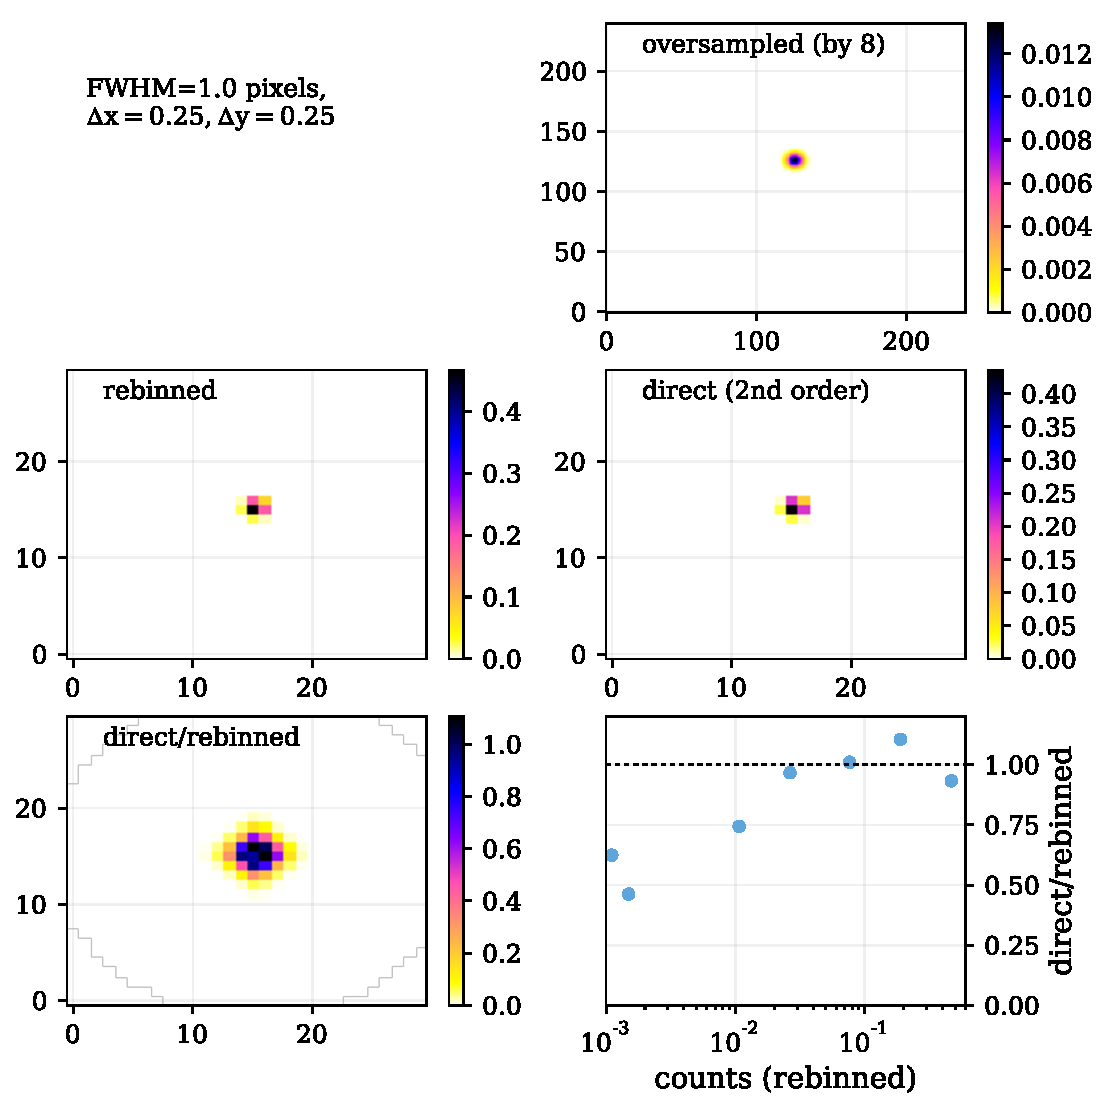
\includegraphics[width=\textwidth]{figures/undersample.pdf}
\caption{A demonstration of the effect of undersampling using a symmetric gaussian PSF with FWHM=1.0 native detector pixels (similar to the undersampling of the F090W PSF). The PSF is shifted 0.25 pixels in both x and y. 
{\it Top Right:} The PSF calculated on a grid oversampled from the native detector pixels by a factor of 8. 
{\it Middle left:} The oversampled PSF rebinned to the native detector pixel grid, giving an accurate reperesentation of the true pixel counts that would be expected for this PSF.  
{\it Middle right:} The PSF calculated directly on the native grid using the 2nd-order approximation to the pixel value.  
{\it Bottom Left:} The ratio of the direct 2nd order calculation to the oversampled and rebinned pixels fluxes, as a function of pixel flux. 
\label{fig:undersample}}
\end{figure}

\begin{figure}
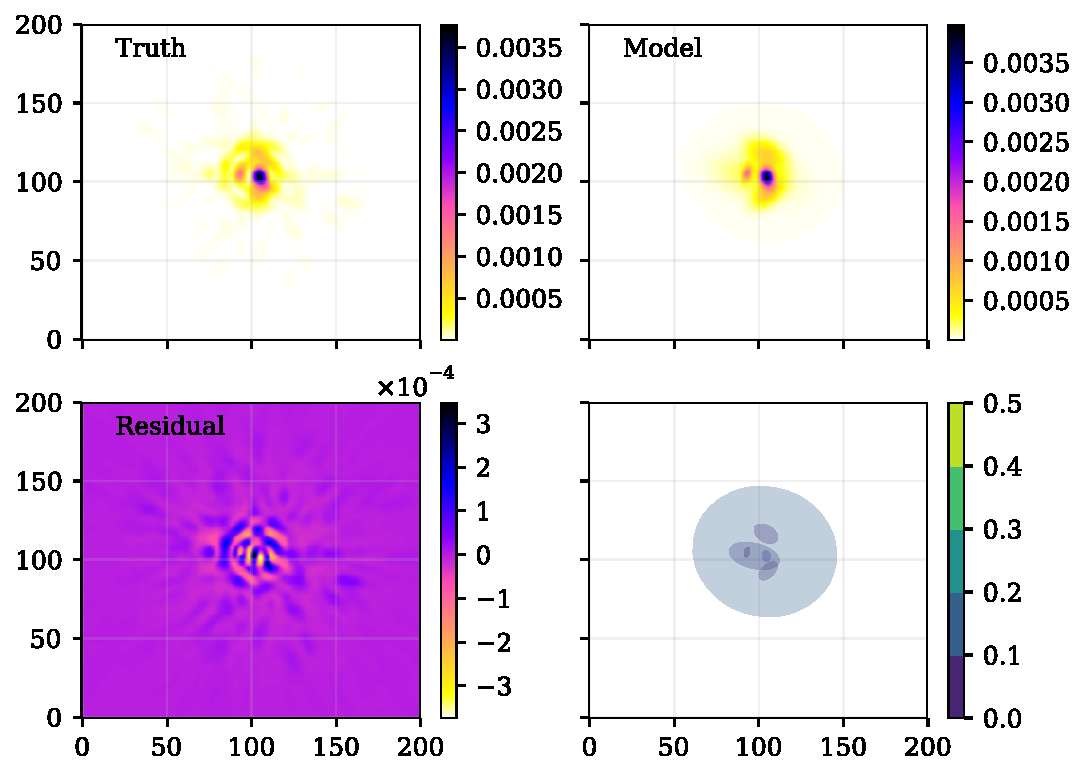
\includegraphics[width=\textwidth]{figures/gm_psf_f090w.pdf}
\caption{A mixture of 6 Gaussians fit to theF090W PSF.  
{\it Top Left:} The input image of the PSF (oversampled by a factor of 8 from the detector pixels) 
{\it Top Right:} The fitted model PSF.  
{\it Bottom Left:} The residual, showing the model PSF subtracted from the input PSF 
{\it Bottom Right:} Ellipses showing the location, sizes, and position angle of the 6 fitted Gaussians, color coded by the total fractional flux of each Gaussian.
\label{fig:psf_mixture}}
\end{figure}

\begin{figure}
\label{fig:sersic}
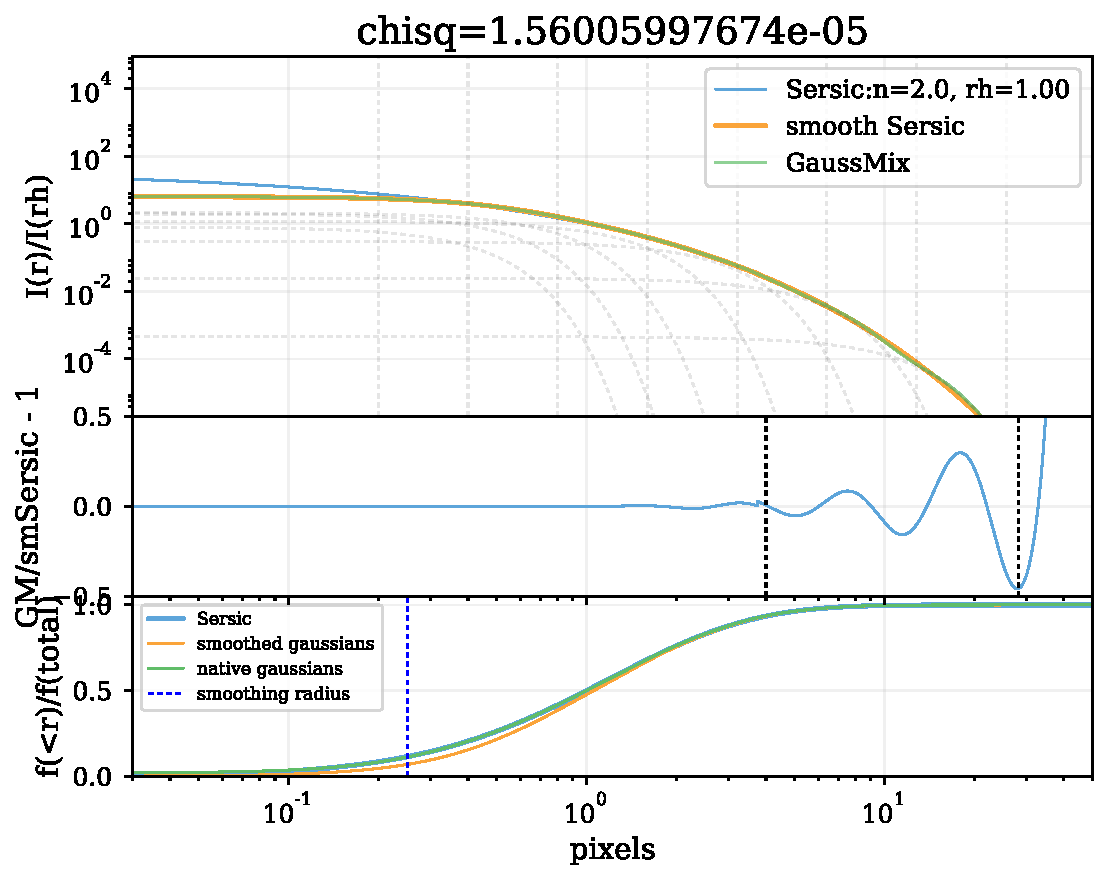
\includegraphics[width=\textwidth]{figures/gm_sersic.pdf}
\caption{A mixture of Gaussians fit to a smoothed Sersic model.  
{\it Top:} Radial surface brightness profiles of the unsmoothed Sersic profile for $n=2, r_h=1$ pixel ({\it blue}), the Sersic profile smoothed with Gaussian of 0.25 pixels dispersion ({\it orange}), and the Gaussian mixture approximation ({\it green}).  
   The vertical dashed lines show the fixed dispersion of each of the zero mean Gaussians used in the approximation, and the dashed curves show the contribution of each Gaussian to the approximated profile.  
{\it Middle:} The fractional profile residual.  
{\it Bottom:} The cumulative flux as a function of radiaus for each profile.
\label{fig:sersic}}
\end{figure}


\begin{figure}
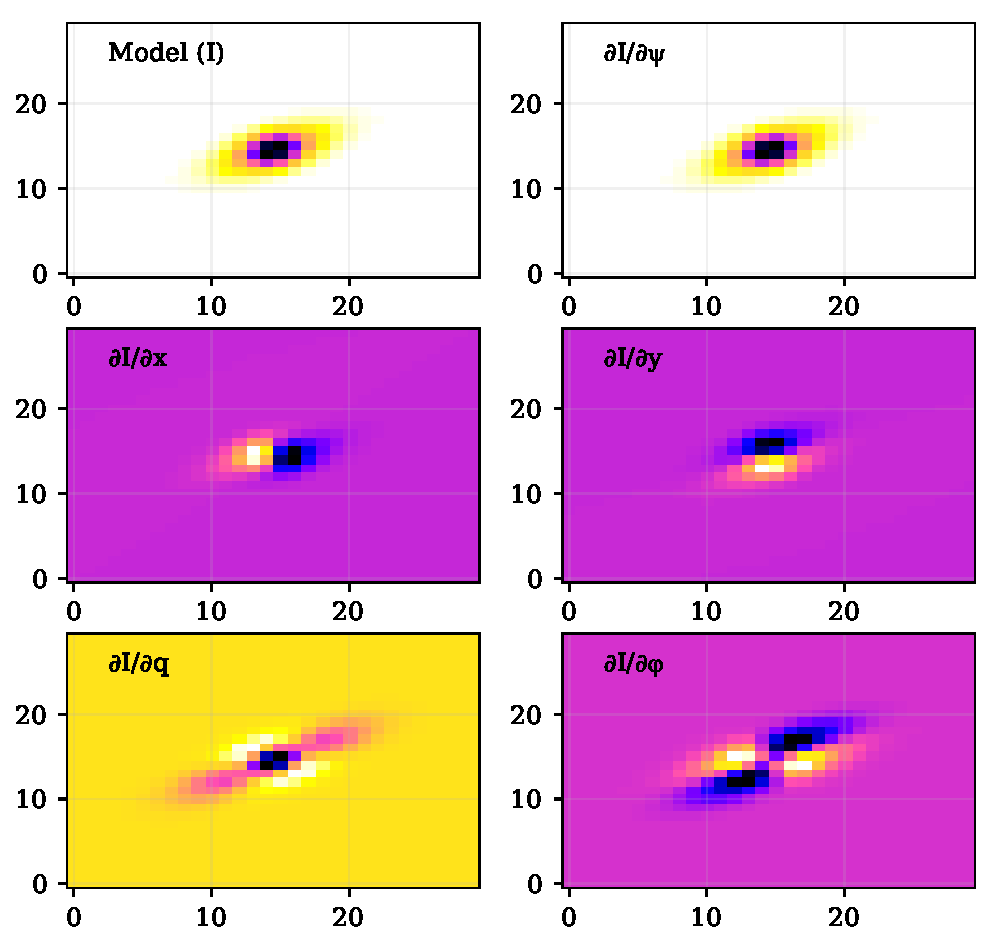
\includegraphics[width=\textwidth]{figures/demo_gaussgal.pdf}
\caption{For a single gaussian PSF and a simple single Gaussian model (with axis ratio $q=0.5$ and position angle $\varphi=30^{\deg}$), this figure shows the model and the image gradients with respect to flux, $x$, $y$, $q$, and $\varphi$.
\label{fig:mock_gal}}
\end{figure}


\begin{figure}
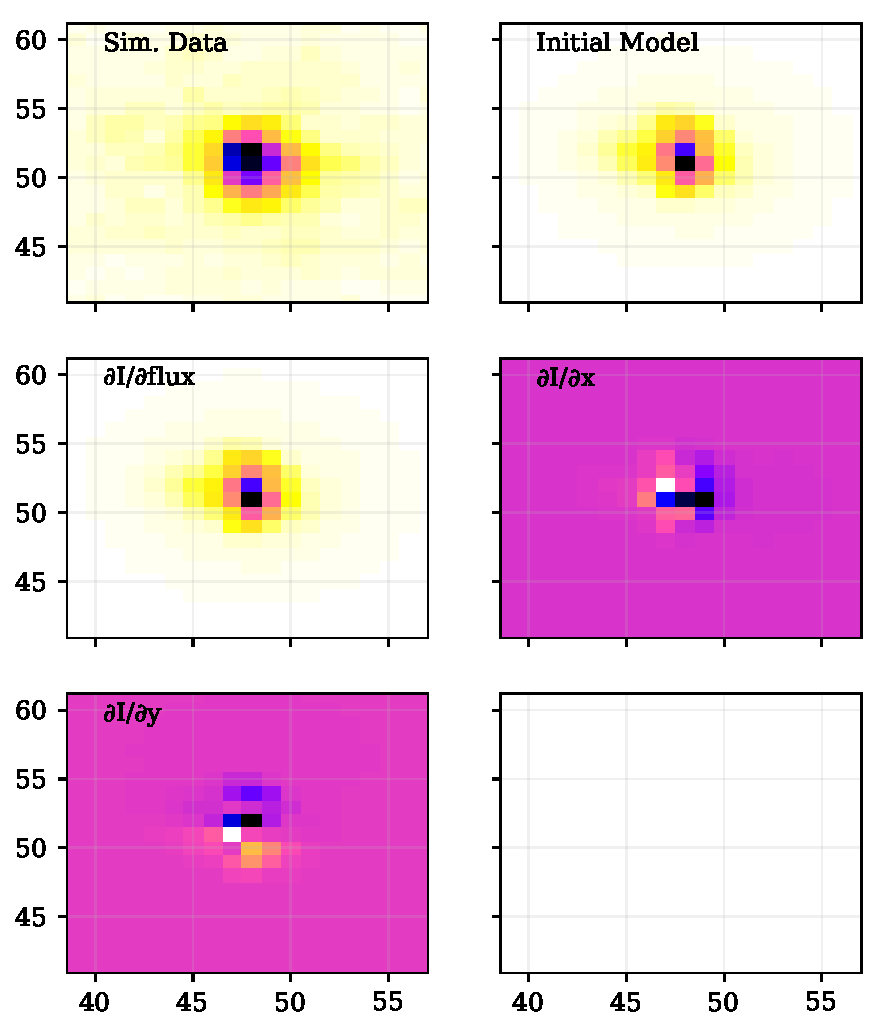
\includegraphics[width=\textwidth]{figures/demo_f090w_pointsource.pdf}
\caption{{\it Top left: } Simulated F090W point source data from CW.  
{\it Top Right:} Initial model guess.  
{\it Succeeding Panels:} Gradient images of the initial model with respect to the 3 point source model parameters.
\label{fig:f090w}}
\end{figure}



\begin{thebibliography}{}\raggedright
\bibitem[Bernstein, \& Jarvis(2002)]{bernstein02}
Bernstein, G.~M., \& Jarvis, M.\ 2002, \aj, 123, 583.

  \bibitem[Greisen et al.(2002)]{greisen02}
Greisen et al. 2002, A\&A 395, 1061

\bibitem[Hogg \& Lang(2013)]{hogg_mog}
Hogg, D.~W. \& Lang, D. 2013, PASP 127, 719

\bibitem[Trujillo et al.(2001)]{trujillo01}
Trujillo, I. et al. 2001, MNRAS 321, 269


\end{thebibliography}


\end{document}